%ex14_fig2.tex
%coloration via l'algo de l'exemple
\begin{figure}[h]
	\begin{center}
	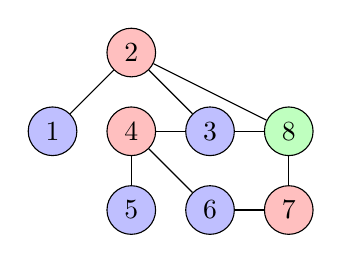
\begin{tikzpicture}
		\node[circle,draw=black,fill=blue!25] (x1) at (0,0) {1};
		\node[circle,draw=black,fill=red!25] (x2) at (1,1) {2}
			edge[-] (x1);
		\node[circle,draw=black,fill=blue!25] (x3) at (2,0) {3}
			edge[-] (x2);
		\node[circle,draw=black,fill=red!25] (x4) at (1,0) {4}
			edge[-] (x3);
		\node[circle,draw=black,fill=blue!25] (x5) at (1,-1) {5}
			edge[-] (x4);
		\node[circle,draw=black,fill=blue!25] (x6) at (2,-1) {6}
			edge[-] (x4);
		\node[circle,draw=black,fill=red!25] (x7) at (3,-1) {7}
			edge[-] (x6);
		\node[circle,draw=black,fill=green!25] (x8) at (3,0) {8}
			edge[-] (x3)
			edge[-] (x2)
			edge[-] (x7);
	\end{tikzpicture}
	\end{center}
	\caption{Coloration par l'algorithme (également optimale)}
	\label{ex24_fig2}
\end{figure}

